\begin{frame}
\frametitle{What do we talk about when we talk about Dirac?}
\begin{columns}
\column{0.35\textwidth}
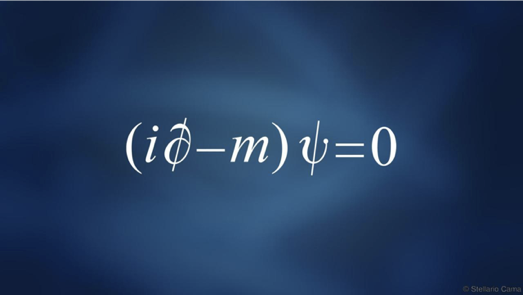
\includegraphics[scale=0.20]{dirac-eq.png}
 
 \column{0.6\textwidth}
%\begin{block}{}
If neutrinos were fermions of spin 1/2 they could presumably described by Dirac equation. Dirac had proposed his famous equation in 1928, two years before the neutrino was proposed by Pauli.  In 1929 P.A.M. Dirac had published his famous paper predicting antimatter (the positron), who would be discovered shortly after by Andersen. Yet, in 1930, antimatter was a concept as fantastic and hard to believe in as the neutrino itself.  

%\end{block}
\end{columns}
\end{frame}
